%% Tópico referente a instalação do Latex

\section{Instalando o \LaTex}

\begin{frame}{Programas necessários}
\begin{itemize}
\item \prog{\TeX\ Live} (Windows, Mac, Linux) ou \prog{MiK\TeX\ } (Windows);
\end{itemize}
\end{frame}

\begin{frame}{Instalando o \TeX{} Live no Linux}
\begin{itemize}
\item Instalador do Ubuntu 11.04 Natty Narwhal:
\end{itemize}


\centering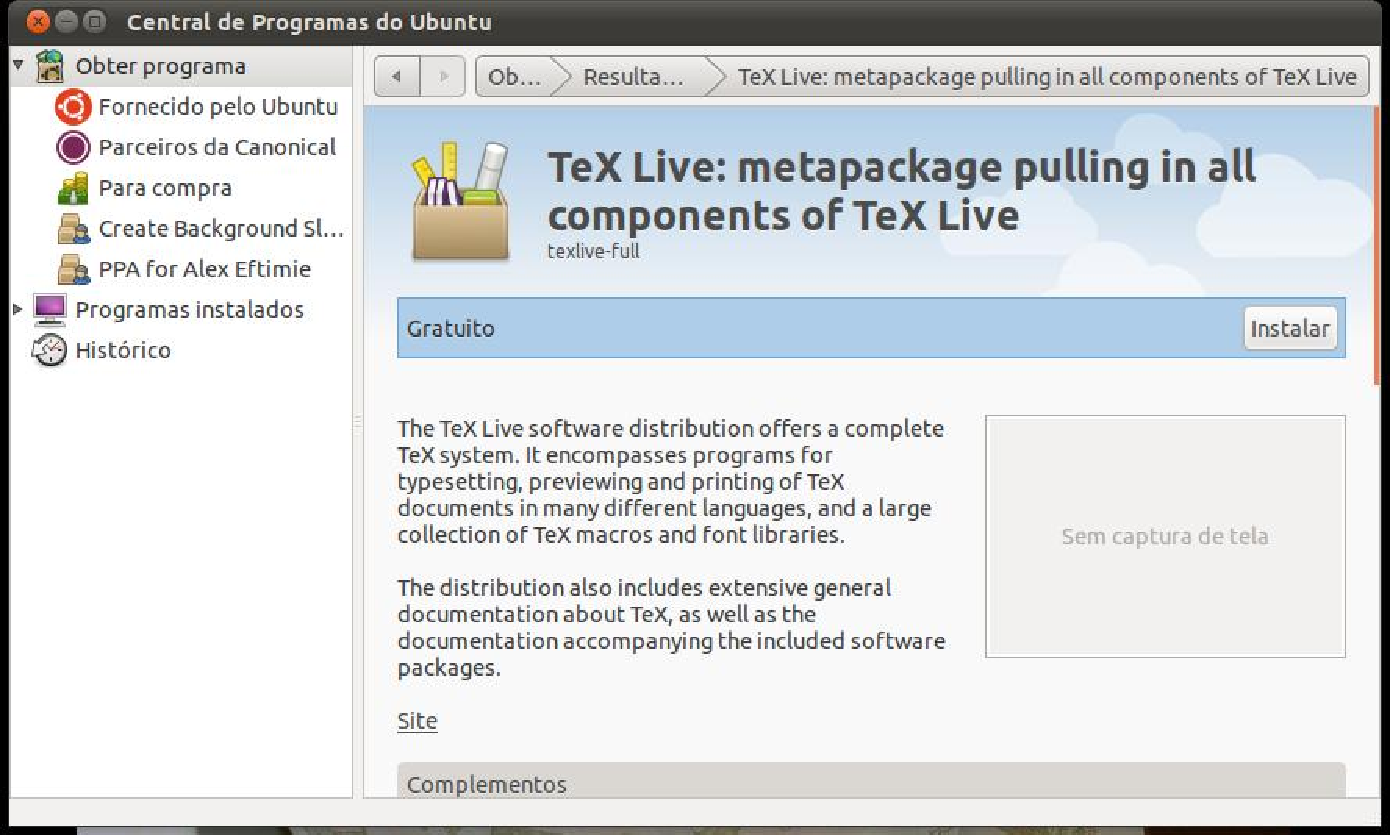
\includegraphics[width=\textwidth,height=.8\textheight,keepaspectratio]{ubuntu}

\end{frame}

%% \begin{frame}{Instalando o \TeX{} Live no Ubuntu-Linux}
%% \begin{itemize}
%% \item O Ubuntu segue as regras do Projeto Debian; Por isso, a instalação da versão \TeX\ Live/Debian é necessária para resolver as dependências  de outros programas Debian, mas esta versão instalada no Ubuntu não é atualizada na mesma velocidade que a produzida para o TUG (\TeX\ Users Group).
%% \item Ambas as instalações podem conviver no mesmo computador. Leia o documento (em italiano):\\
%% {\small\url{http://profs.sci.univr.it/~gregorio/texlive-ubuntu.pdf}}
%% \item Na instalação deve-se assegurar que a data da versão de \TeX\ Live seja sempre a mais recente, e essa é a versão que deve ser usada na preparação de documentos.
%% \end{itemize}
%% \end{frame}

\begin{frame}{Instalando o \TeX{} Live no Ubuntu-Linux}
\begin{block}{Console}
 Usando o apt-get:\\
 apt-get install texlive-full
\end{block}

\begin{block}{Arquivos e mirrors internacionais}
\begin{itemize}
\item O programa de instalação é:
\url{http://mirror.ctan.org/systems/texlive/tlnet/install-tl-unx.tar.gz}

\item Existem muitos mirrors internacionais; veja:
\url{http://ctan.org/mirrors}

\item A instalação de um mirror é preferível já que, geralmente, é mais rápida.
\end{itemize}
\end{block}
\end{frame}

\begin{frame}{\TeX\ Live para MacOS}
\begin{itemize}
\item As máquinas MacOS precisam de uma versão particular do \TeX~Live que chama-se \prog{Mac\TeX}.
\item Veja: \url{http://www.tug.org/mactex/}
\item As instruções são mais simples que em outros sistemas e a instalação é mais rápida.
\end{itemize}
\end{frame}

\begin{frame}{Instalando MiK\TeX\ no Windows}
MiK\TeX\ oferece duas instalações:
\begin{itemize}
\item Instalação básica, que permite instalar os pacotes que faltam, 
quando necessário;
\item Instalação completa (preferível).
\end{itemize}

\end{frame}

\begin{frame}{Instalação da versão MiK\TeX\ básica}
\centering
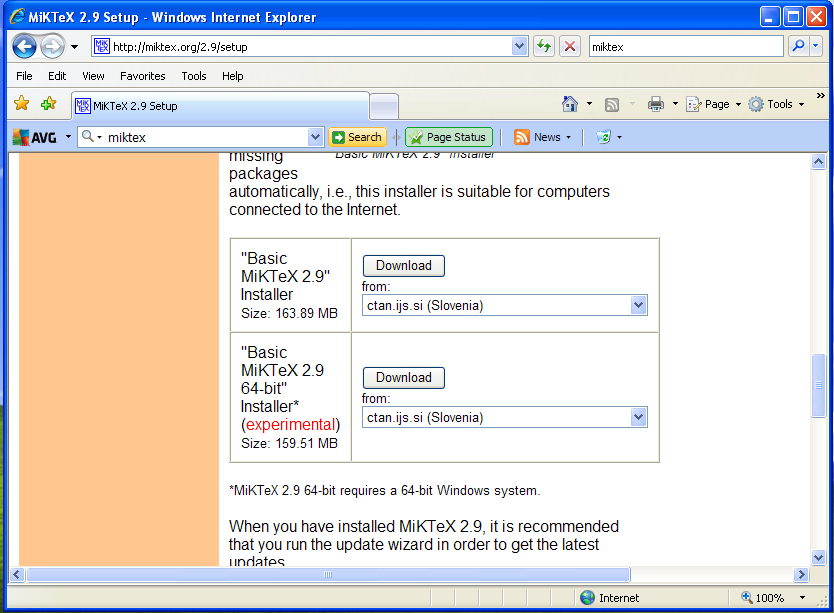
\includegraphics[width=\textwidth,height=\textheight,keepaspectratio]{MiKTeX-Basic}
\end{frame}

\begin{frame}{Instalação da versão MiK\TeX\ completa}
\centering
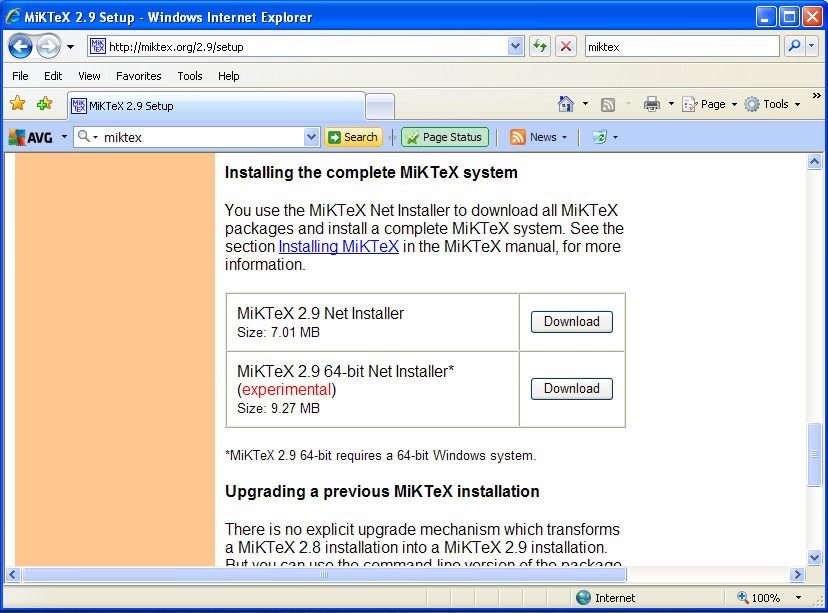
\includegraphics[width=\textwidth,height=\textheight,keepaspectratio]{MiKTeX-Complete}
\end{frame}
